%# -*- coding: utf-8-unix -*-
% !TEX program = xelatex
% !TEX root = ../thesis.tex
% !TEX encoding = UTF-8 Unicode
%%==================================================
%% chapter02.tex for SJTU Master Thesis
%% based on CASthesis
%% modified by wei.jianwen@gmail.com
%% Encoding: UTF-8
%%==================================================

\chapter{基于深度强化学习的NL2SQL生成}
\label{chap:enl2sql}

\section{研究问题}
\section{相关技术}
\section{解决方案}



给定一个输入自然语言问题,我们的目标是生成相应的SQL查询。在下文和整篇论文中,我们使用WikiSQL数据集(Zhong et al。,2017)作为我们的激励示例。但是,应该注意的是,我们的方法通常适用于其他NL2SQL数据,可以正确选择操作清单并重新设计解析器状态。

WikiSQL数据集包含80,654对问题和SQL查询,分布在维基百科的24,241个表中。与自然语言问题一起,输入还包含单个表模式(即表列名称)。每个表只存在于一个拆分(火车,开发或测试)中,这要求模型推广到看不见的表。图1显示了一个示例。 WikiSQL数据集查询的SQL结构受到限制,并始终遵循模板SELECT agg selcol WHERE col op val(AND col op val)*。在这里,selcol是一个

单表列和agg是聚合器(例如,COUNT,SUM,空)。 WHERE段是一系列连接过滤条件。每个op是过滤运算符(例如,=),并且在问题中提到过滤值val。虽然数据集带有条件的“标准”线性排序,但鉴于AND的语义,顺序实际上是无关紧要的。

在整篇论文中,我们将解析器的输入表示为x。它由带有标记wi的自然语言问题w和具有列名称cj的单个表模式c组成。列名称cj可以包含一个或多个标记。解析器需要生成可执行的SQL查询y作为其输出。

给定输入x,结构化输出y的生成被分解为一系列解析决策。 解析器从初始状态开始,并根据学习的策略逐步采取操作。 每个动作都将解析器从一个状态推进到另一个状态,直到它到达终端状态之一,在那里我们可以提取完整的逻辑形式y。 我们采用概率方法
塑造政策。 它在给定输入x和运行的解码历史的情况下预测有效的后续动作集合上的概率分布。 然后,训练这种增量语义解析器的目标是优化该参数化策略。

\begin{figure}[!htp]
  \centering
  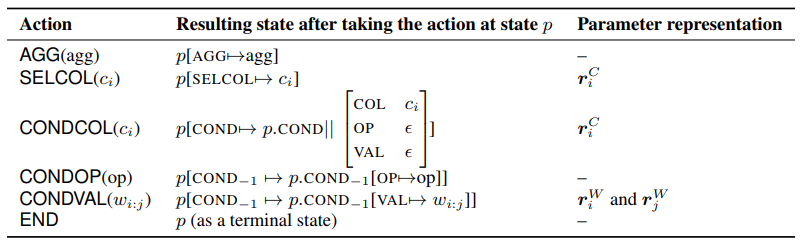
\includegraphics[width=20cm]{example/incsql.png}
  \bicaption[这里将出现在插图索引中]
    {中文题图}
    {English caption}
  \label{fig:SRR}
\end{figure}



965/5000
形式上,我们让Pθ(y | x)=Pθ(a | x),其中θ是模型参数。 执行动作序列a = {a1,a2,...。。 ,ak}将解析器从初始状态引导到包含解析结果y的终端状态。 这里我们假设每个y只有一个相应的动作序列a,我们将在第4节重新讨论这个假设。动作序列的概率被进一步考虑为增量决策概率的乘积:Pθ(a | x)= Qk i = 1Pθ(ai | x,a <i),其中| a | = k。
在推理期间,我们的解码器不是试图枚举整个输出空间并找到最高得分a * = arg maxaPθ(a | x),而是采用贪婪的方法:在每个中间步骤,它根据以下方式选择最高的得分行动: 政策:a *
i = arg maxaiPθ(ai
| x,a *
<I)。
在以下小节中,我们定义解析器状态和动作清单,然后描述编码器 - 解码器神经网络模型体系结构。


我们的解码器的主要组成部分是对概率分布Pθ(a | x,a <i)进行模拟
解析器动作以输入x和过去动作a <i为条件。它有两个主要挑战:
(1)没有固定的有效解析器动作集:它取决于输入和当前解析器状态;
(2)解析器决策依赖于上下文:它依赖于解码历史和信息
嵌入在输入问题和列标题中。
我们采用基于LSTM的解码器框架,通过个人解决第一个挑战
行动得分。该模型将每个候选动作a评分为sa并使用softmax函数
将分数标准化为概率分布。在时间步骤i,我们表示隐藏的当前解码器
以h为状态
\section{实验与分析}
\section{本章小结}